\section{Comparison with Experiments}\label{sec:validity}
\begin{figure}[t]
\centering
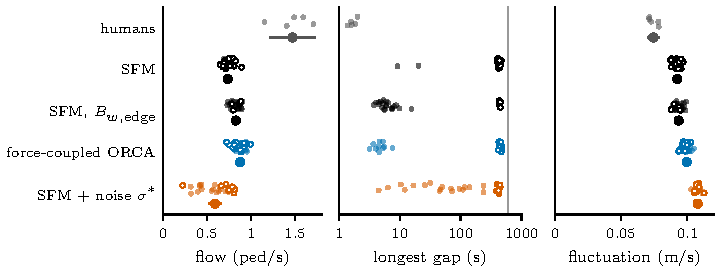
\includegraphics[width=\textwidth]{../figures/fig8_croma.pdf}
\caption{Flow, longest gap between passages (log scale) and waiting-zone velocity fluctuation at the CroMa entrance ($w=0.8$\,m) for five human runs and 25 runs per model variant (means and 95\% intervals for flow and fluctuation). Open markers: runs that did not complete, whose final gap is right-censored at the 600\,s horizon; filled markers: longest gap of completed runs.}
\label{fig:croma}
\end{figure}
%
\subsubsection{Experiments and Model Runs.}
The CroMa bottleneck experiments~\cite{fzj_ped20219,boomers2023data} include five runs through a 0.8\,m wide bottleneck: two with a straight bottleneck 2.0\,m long (4D030, 4D040; its walls, thin in the model, taper to a wedge in their second metre) and three with one 0.2\,m long, a door in a wall (4D110, 4D120, 4D130). The five runs mix three motivation conditions: participants walked normally (4D030, 4D110), hurried (4D040, 4D120) or gave full commitment (4D130). Except in 4D130 they kept a 2\,m semicircle before the bottleneck clear.
%C2: A9 motivation-condition breakdown (flow per condition)
The trajectories are published under CC BY 4.0~\cite{fzj_ped20219}.
%C2: A9 (vi) ethics-approval sentence of the experiments
All tracked participants, \RevDFourDonethirtyPassed--\RevDFourDthirtyPassed\ per run, pass the entrance and none deadlocks (duplicate track IDs in 4D040 and 4D110 merged).

Measured bottleneck flow grows with width~\cite{hoogendoorn2005,seyfried2009}, so the model runs use the CroMa geometry (Sect.~\ref{sec:geometry}). Each human run has five model runs (25 per variant), with as many agents as participants passed, starting at rest farther from the entrance. Four variants ran for up to 600\,s with uncalibrated default parameters: SFM; SFM with the jamb range $B_{w,\rm edge}$; force-coupled ORCA (RVO2); and SFM+noise $\sigma^\ast$ (Sect.~\ref{sec:att-whole}).
%C2: A9 agent radii about 10% larger than the participants' (number needed)

A run's flow is the number of passages through the entrance plane less one over the time from the first to the last passage, counted up to any deadlock. The flow ratio of a variant is the mean flow of its 25 runs over the mean flow of the five human runs, with a 95\% interval from the log ratio (Welch $t$, unadjusted). A run is censored when it deadlocks or still runs at 600\,s: its final gap is right-censored there, so we report the longest gap of completed runs and the number of censored runs separately. The velocity fluctuation is the standard deviation of agents' smoothed velocities relative to neighbours within 0.74\,m, in the waiting zone (Fig.~\ref{fig:geometry}, H) while its mean speed is below 0.3\,m/s.

\subsubsection{Flow, Gaps and Velocity Fluctuation.}
Between the 10\% and the 90\% passage humans pass \PendHumanWindowFlow\,ped/s and the model \RevDThreeCOneWindowFlow\,ped/s (SFM) to \RevDThreeCThreeWindowFlow\,ped/s (force-coupled ORCA). Over whole runs the human flow is \PendHumanFlow\ [\PendHumanFlowLo, \PendHumanFlowHi]\,ped/s, and the fastest model run (\PendModelFlowMax\,ped/s) is slower than the slowest human run (\PendHumanFlowMin\,ped/s). With the 2.0\,m bottleneck humans pass \PendLongHumanFlow\,ped/s and the model \RevDThreeCSigLongFlow--\RevDThreeCThreeLongFlow\,ped/s; with the 0.2\,m bottleneck, \PendShortHumanFlow\ and \RevDThreeCSigShortFlow--\RevDThreeCThreeShortFlow\,ped/s. The longest human gap averages \EtenHumanGap\,s, and its maximum is \EtenHumanGapMax\,s at the 0.01\,s resolution of the gap data; \EtenHumanGapsOverTwoTotal\ gap in the five runs exceeds 2\,s.

Model passages come in bursts, with \PendCThreeGapsTwo--\PendSigGapsTwo\ gaps longer than 2\,s per run (Fig.~\ref{fig:croma}). Per variant, of 25 runs:
\begin{center}\scriptsize\setlength{\tabcolsep}{3pt}
\begin{tabular}{@{}lcccccc@{}}
\toprule
Variant & Complete & Deadlock & Running & Censored & Max.\ gap & Flow ratio [95\%]\\
\midrule
SFM & \RevDThreeCOneComplete & \RevDThreeCOneDeadlock & \RevDThreeCOneCapped & \RevDThreeCOneCens & \PendCOneGapCompleteMax\,s & \RevDThreeCOneFlowRatio\ [\RevDThreeCOneFlowRatioLo, \RevDThreeCOneFlowRatioHi]\\
Jamb range & \RevDThreeCEdgeComplete & \RevDThreeCEdgeDeadlock & \RevDThreeCEdgeCapped & \RevDThreeCEdgeCens & \PendCEdgeGapCompleteMax\,s & \RevDThreeCEdgeFlowRatio\ [\RevDThreeCEdgeFlowRatioLo, \RevDThreeCEdgeFlowRatioHi]\\
Force-coupled ORCA & \RevDThreeCThreeComplete & \RevDThreeCThreeDeadlock & \RevDThreeCThreeCapped & \RevDThreeCThreeCens & \PendCThreeGapCompleteMax\,s & \RevDThreeCThreeFlowRatio\ [\RevDThreeCThreeFlowRatioLo, \RevDThreeCThreeFlowRatioHi]\\
Noise $\sigma^\ast$ & \RevDThreeCSigComplete & \RevDThreeCSigDeadlock & \RevDThreeCSigCapped & \RevDThreeCSigCens & \PendSigGapCompleteMax\,s & \RevDThreeCSigFlowRatio\ [\RevDThreeCSigFlowRatioLo, \RevDThreeCSigFlowRatioHi]\\
\bottomrule
\end{tabular}
\end{center}
Running: still moving at 600\,s; censored: deadlocked or running; max.\ gap: longest gap of completed runs. The Kaplan--Meier median longest gap is \RevDThreeCEdgeGapKMMedian\,s (jamb range) and \PendSigGapKMMedian\,s (noise), and at least \PendCOneGapLowerMedianTwo\ and \PendCThreeGapLowerMedianTwo\,s for SFM and force-coupled ORCA. The model's velocity fluctuation (\RevDThreeCOneFluct--\PendSigFluct\,m/s) exceeds the human one, \EtenHumanFluct\ [\EtenHumanFluctLo, \EtenHumanFluctHi]\,m/s.

With uncalibrated default parameters every variant passes \RevDThreeRatioMin--\RevDThreeRatioMax\ of the human flow at this width.
%C2: B1 throttle-off CroMa flow (one sentence: flow ratio with the Eq. (2) density throttle off)
The cause of the deficit is not identified here.
